\chapter{绪论}
\label{chap:references}

\section{引言}

操作系统的“Page Fault”异常处理例程首先会判断,该数据的虚拟地址是否是该任务的合法地址?根据之前操作系统的设置,答案是“Yes”;抛出异常之后, 内核取出保存在相应页表项中地址,通过地址转换将获取虚拟地址的物理地址;后把对应的物理页号写入页表项,把页表项中的存在位设“1”;最后,返回该任务,让该任务重新执行访问数据的指令。此时, 处理器再次执行这条指令,块表还是没有相应的页表项信息,而对应页表项内容合法,所以块表会发生缓存操作,并完成地址转换,实现访问数据指令的执行。

相对于内存访问,交换区的扇区访问要慢很多。为了进一步提高系统的执行效率,当操作系统在让存储设备进行I/O访问时,可将当前任务设置为阻塞状态,并切换其他可以运行的任务继续执行。通过这种任务调度方式,可以充分发挥多道程序和分时多任务的整体执行效率

本文的工作利用Rust的语言优势来重新设计操作系统内核并尝试为其添加异步特性。 毕设将围绕异步进行操作系统的调度设计,期望为操作系统内核异步设计积累经验和提供有所裨益的思路。

\section{研究背景与意义}

研究目的:异步的提出是为了提高程序在热点事件下的并发性能。

研究意义:编译器与操作系统进行密切配合,用户态的异步系统调用会同编译器自动生成相应的系统调用请求代码和协程控制块数据结构;只有在第一次系统调用和最后一次系统调用时需要进入内核空间;中间各次的系统调用只进行系统调用结果查询和进程、线程或协程切换。

研究好处:异步调度下,操作系统应对高并发的任务时,可以获得更好的响应表现,CPU可以一直处在忙碌的状态。无栈的协程,内部的状态转换通过状态机图实现,无需函数主动调用yield,内部也只是状态的转换,无需多余的栈空间开销。

\section{国内外研究现状}

\subsection{国外现状}
国外异步操作系统的研究以Linux为主,其中以libaio和io\_uring的研究比价典型。以下是这两种情况的简要阐述。

\subsubsection{Libaio}
\begin{figure}[htb]
    \figureCapSet
    \centering
    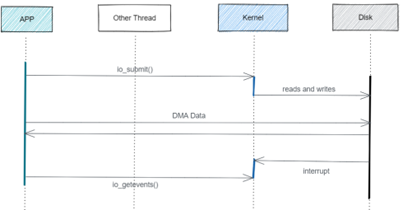
\includegraphics[width=.8\linewidth]{figure/c1/libaio.png}
    \caption{Libaio\pagescite{IoUring1}的工作流}
    \label{figure:c1libaio}
\end{figure}

Libaio的工作流如\autoref{figure:c1libaio}所示, 以read的请求来说, direct IO\pagescite{IoUring1}的模式会把从磁盘上读取的数据直接返回给了用户态的内存空间,不会在内核中缓存,当存在多次重复读取的场景,每次都需要读取磁盘,这样会增加磁盘的压力。


\subsubsection{IO\_URING}
\begin{figure}[htb]
    \figureCapSet
    \centering
    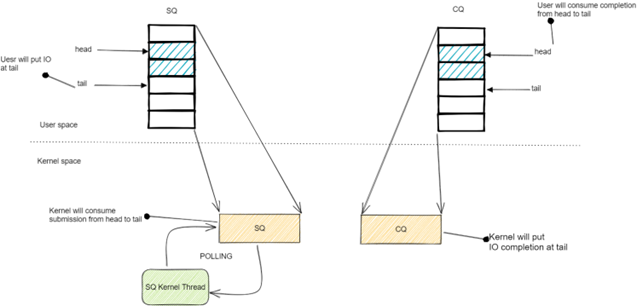
\includegraphics[width=.8\linewidth]{figure/c1/iouring.png}
    \caption{io\_uring\pagescite{IoUring2}的工作流}
    \label{figure:c1iouring}
\end{figure}

io\_uring的工作流如\autoref{figure:c1iouring}所示,io\_uring的基本逻辑与linux-aio\pagescite{IoUring2}是类似的,提供两个接口,一个将I/O请求提交到内核,一个从内核接收完整的事件。但是在设计上是真正的异步。通过参数,通过系统调用,将请求放入请求队列,不会做额外的工作,保证了应用不会被阻塞。io\_uring无需像aio那样使用 poll+read/write来处理sockets,只需要提交一个阻塞式的度,请求完成之后,就会出现在CQ(completion ring)。io\_uring实例在设计上有两个环形队列,请求队列和完成队列,使其能在内核空间和用户空间之间共享, 两者都是单生产者、单消费者,提供无锁的接口,内部使用内存屏障同步。

\textbf{io\_uring可以工作在三种模式上}
\begin{enumerate}
\item 中断驱动的默认模式。提交相应的I/O请求,查询完成队列的状态判断是否完成。
\item 轮询模式,通过文件系统和块设备支持轮询作为基础,相比前一种模式,虽然延迟比较低,但会消耗更多计算资源。当一个读或写请求提交给轮询上下文之后,应用必须轮询CQ队列,判断请求是否已经完成。
\item 内核轮询模式,会创建一个内核线程来执行请求队列的轮询工作\pagescite{IoUring1}。
\end{enumerate}

io\_uring的内核轮询模式, 使得用户空间的应用无需切到到内核态就可以触发I/O的操作\pagescite{IoUring0}。通过请求队列来提交请求事件,以及监控完成队列的状态,无需系统调用,就能提交和捕获I/O操作\pagescite{IoUring0}。


\subsection{国内现状}

国内则主要是基于国外设计的一些探索, 如下是比较典型的共享调度器的设计,内核和用户的调度资源被存储在统一共享队列,由队列缓冲同步数据,达到异步并发的现实需求。

\subsubsection{tornado-os的调度器}
\begin{figure}[htb]
    \figureCapSet
    \centering
    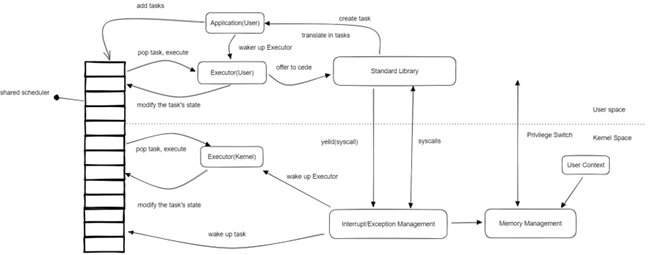
\includegraphics[width=.8\linewidth]{figure/c1/sharedscheduler.png}
    \caption{shared\_scheduler\pagescite{tornado0}的工作流}
    \label{figure:c1sharedscheduler}
\end{figure}

调度器被同时暴露在内核空间和用户空间, 这将所使用的代码、任务资源都在内核和用户之间共享。用户和内核拥有近乎相同的异步调度逻辑。即从共享的任务池中接收任务并执行。

总结一下国内与国外的研究情况。基本上,异步系统调用的执行过程应当符合如下设计,
\begin{enumerate}
    \item 第一次异步系统调用时
    \begin{itemize}
        \item 用户进程准备系统调用参数、发出系统调用请求;
        \item 内核进程将映射共享内存、发起相应服务协程的异步执行;
        \item 内核进程执行完服务协程后,再响应队列保存返回值,并通过用户态中断通知应用进程;
    \end{itemize}
    \item 第二次异步系统调用时
    \begin {itemize}
        \item 用户进程再请求队列转杯系统调用参数;在共享内存的响应队列中查看一次系统调用的结果;
        \item 内核进程在完成第一个服务协程后,在共享内存的响应队列中保存返回值,主动查询新的系统调用请求,并执行;如果没有新的请求,则让出CPU;
    \end{itemize}
\end{enumerate}

如何开辟缓冲队列,执行轮询,实现异步工作,是异步设计的重点。

\section{研究的目标与内容}

\subsection{研究的目标}

程序有执行独立的正交化的任务,彼此之间无需串行执行。例如,现代的网络服务器可以同时监听并响应大量的客户端请求。宏观而言,对于每个请求,服务器的响应无需按照某个特定的处理顺序,理论上每个请求可以被当作独立的执行单元,并行执行。当操作系统的底层服务并发提供支持,则网络服务程序会有更好的性能表现。

本文的工作主要利用Rust语言优势来重新设计操作系统内核并尝试为其添加异步的特性。

\subsection{研究的内容}

操作系统内核,为了提升线程的性能,基于编程架构,系统尝试在应用层复用线程资源,由此引出协程。毕设工作尝试使得操作系统中不同资源被调度器所共享,调度器使得资源同时共享给内核和用户,两者将拥有近乎相同的调度处理机制,同时,为了降低系统的耦合程度,尝试模块化系统内核,尝试将系统组件剥离。所以,本文尝试以下工作:

本文将实现一个ring\_scheduler,用来作为调度的缓冲队列,内核和用户的任务,将会以指针的方式存储在缓冲队列中。

本文尝试将从理论上构建一个依赖库,将杂糅在一起的内核模块,通过Cargo的编译形成一个依赖树,从而更好管理和开发系统内核。

\section{论文的组织安排}

本文的组织结构如下:

第一章, 介绍了操作系统异步调度设计的研究背景,意义,相关的国内外研究现状,由此确定了研究的目标与内容。

第二章, 介绍开发系统软件时,所需要具备的一些理论和技术支持,对Rust\pagescite{rust0}语言、riscv\pagescite{riscv0}和异步设计做了阐述。

第三章, 详细描述了系统的设计, 从异步调度、模块设计两个个方面设计系统。

第四章, 对系统的部分实现进行解释,遵循系统设计,依次对部分代码进行阐述。

第五章, 总结了本文工作的大致内容,自己在开发过程中的一些难点和相关的一些经验,同时提出了对本文系统设计改进的些许展望。
